\documentclass[12pt, a4paper]{article}

%%------------------Preamble------------------%%

    %% 引入Package %%
\usepackage[margin=2cm]{geometry} % 上下左右距離邊緣3cm
\usepackage{fancyhdr}   % 頁首頁尾 fancy header
\usepackage{titling}    % 設定 title,author,date
\usepackage{mathtools,amsthm,amssymb} % 引入 AMS 數學環境
\usepackage[shortlabels,inline]{enumitem} %加強 enumerate, itemize 功能
\usepackage{setspace}
\usepackage{tcolorbox}
\usepackage{xcolor} % 用於表格上色
\usepackage{graphicx}      % 用於縮放表格寬度
\usepackage{array}
\usepackage{float} % for [H] float placement
\tcbuselibrary{breakable}
\usepackage{tabularx}
\usepackage{colortbl}

%% 中文環境，僅限使用 XeLaTeX 編譯器 %%

\usepackage[CJKmath=true,AutoFakeBold=3,AutoFakeSlant=.2]{xeCJK}

\setCJKmainfont{Noto Serif CJK TC}
\setCJKsansfont{Noto Sans CJK TC}
\setCJKmonofont{Noto Sans Mono CJK TC}

\newCJKfontfamily\Kai{Noto Serif CJK TC}
\newCJKfontfamily\Hei{Noto Sans CJK TC}
\newCJKfontfamily\NewMing{Noto Serif CJK TC}

\XeTeXlinebreaklocale "zh"





\begin{document}

\title{T1 選擇題解答} % 設定標題
\author{李原廷} % 設定作者
\date{\today} % 設定完成日期，也可以使用 \date{\today}

\maketitle

\begin{enumerate}
    \item 衡量所得分配不均度的指標「大島指數」（Oshima index），其定義為？
        \begin{enumerate}[label=\Alph*.]
            \item 所得最高前10\%者之所得，占所有人口（家計單位）所得之比例
            \item 所得5等分位組，最高組的所得除以最低組的所得而得出之倍數
            \item 中位數所得除以平均所得
            \item 所得最高前10\%者的所得除以平均所得。
        \end{enumerate}
        解答：大島指數（五等分位所得差距倍數）：將家戶依據所得分成五個組別，每個組別有20\%的家戶，將所的最高組別的所得除以所得最低組別的所得即為差距倍數，\textcolor{red}{倍數越高}，代表\textcolor{red}{所得分配越不均}。

    \item 下列有關拉弗曲線（Laffer curve）之敘述，何者正確？
        \begin{enumerate}[label=\Alph*.]
            \item 橫軸為稅基，縱軸為稅收的關係
            \item 呈現稅收隨著稅基增加而增加的關係
            \item 可說明課稅影響勞動供給者的工作意願
            \item 在拉弗曲線前段，當稅基增加1\%，納稅人所需負擔的稅負增加大於1\%。
        \end{enumerate}
        解答：
        \begin{figure}[H]
            \centering
            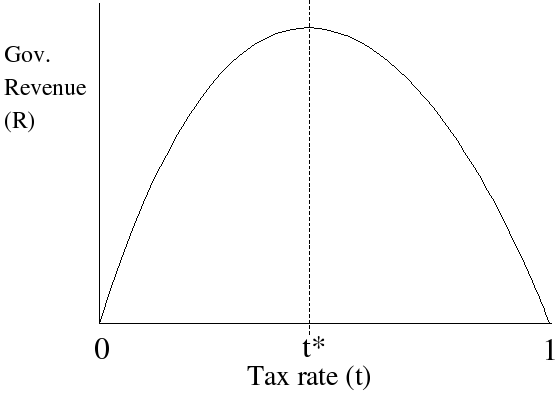
\includegraphics[width=0.5\linewidth]{Laffer Curve.png}
        \end{figure}
        當稅率提高時，會產生「替代效果」，降低人們（勞動供給者）的工作意願（因為稅後報酬減少，休閒的相對成本變低）。當稅率高到某個程度，因為大家不願意工作或選擇逃漏稅，導致「稅基」大幅縮小，最後總稅收反而下降。

    \newpage

    \item 下列何者不是政府財政的主要功能？
        \begin{enumerate}[label=\Alph*.]
            \item 穩定功能
            \item 分配功能
            \item 配置功能
            \item 司法功能。
        \end{enumerate}
        解答：現在政府財政有三個功能：資源配置、所得分配、經濟穩定。即馬斯葛列夫（R. A. Musgrave）所謂政府的三項財政功能。

    \item 福利經濟學第一定理主要在強調經濟資源配置效率與下列何者之關係？
        \begin{enumerate}[label=\Alph*.]
            \item 租稅公平
            \item 社會福利
            \item 完全競爭市場
            \item 政府存在。
        \end{enumerate}
        解答：所有生產者與消費者為完全競爭者，即市場的所有人都是價格接受者，沒有人有市場力量。每一種商品都有市場的存在。在給定這些假設之下，我們可以得出競爭市場機制將導致柏瑞圖效率（Pareto efficiency），即完全競爭市場均衡就是柏瑞圖最適（Pareto Optimality）。

    \item 下列有關古典財政理論的敘述，何者正確？
        \begin{enumerate}[label=\Alph*.]
            \item 主張政府應積極介入市場經濟
            \item 反對國家發行公債
            \item 贊成以貨幣政策調節產出
            \item 主張國家生產體說。
        \end{enumerate}
        解答：古典學派在思想上是個人主義；經濟政策上是自由經濟；財政理論是國家消費體說。主張自由放任，政府不要干預市場的經濟活動，理論整理如下：
        \begin{itemize}
            \item 經費縮小論
            \item 租稅中立論
            \item 公債破產論：反對發行公債，不論對消費支出與資本支出均反對
            \item 健全財政---均衡預算
        \end{itemize}

    \item 福利經濟學第二定理主要在闡述下列何種經濟概念？
        \begin{enumerate}[label=\Alph*.]
            \item 所有消費者的邊際替代率均會相等
            \item 所有生產者的邊際技術替代率均會相等
            \item 完全競爭市場將會引導資源的配置效率
            \item 可在不損及經濟效率下，達成分配公平。
        \end{enumerate}
        解答：福利經濟學第二定理指出，資源的配置效率可以在一個適當的稟賦配置之下，透過自由競爭市場來達成。即社會在原有的適當財產分配之下，讓人們彼此自由交易，就可以達成資源的柏瑞圖效率分配。

    \newpage

    \item 下列何項敘述乃屬規範經濟學所探討之議題？
        \begin{enumerate}[label=\Alph*.]
            \item 對菸酒課稅的價格可能提高
            \item 對菸酒課稅，菸酒的需求量可能減少
            \item 對菸酒課稅，低所得對菸酒的消費比重可能增加
            \item 對菸酒課稅，是否有助所得分配更公平。
        \end{enumerate}
        解答：
        \begin{itemize}
            \item 規範經濟學：主要以「主觀」角度，分析經濟事件發生之好壞評斷，不僅僅是敘述事件因果；從不同角度或不同分析者，可能得出不同的結論。
            \item 實證經濟學：主要以「客觀」角度，描述經濟事件發生之實際狀況，不加入任何應否之評斷；從不同角度或不同分析者，皆可得出一樣的結論。
        \end{itemize}

    \item 下列何者屬於財政學理論提及的政府配置功能？
        \begin{enumerate}[label=\Alph*.]
            \item 補貼低所得家庭健保費
            \item 課徵累進所得稅
            \item 建置交通運輸系統
            \item 維持物價穩定。
        \end{enumerate}
        解答：
        \begin{itemize}
            \item 資源配置功能：指政府為了修正「市場失靈」（如公共財、外部性、自然獨占等問題），介入市場以提高資源使用效率。
            \item 所得分配功能：指政府透過租稅與移轉性支出，來改善市場經濟運作下可能產生的貧富不均，以達到社會公平。\\
            A. 補貼低所得家庭健保費（移轉性支出）屬於此功能。\\
            B. 課徵累進所得稅（租稅政策）屬於此功能。
            \item 經濟穩定功能：指政府透過財政或貨幣政策，來達成充分就業、維持物價穩定、促進經濟成長等總體經濟目標。\\
            D. 維持物價穩定 屬於此功能。
        \end{itemize}

    \item 依據蓋布瑞斯的論點，下列敘述何者正確？
        \begin{enumerate}[label=\Alph*.]
            \item 應適當分配公共財與私有財以達到社會平衡
            \item 導致社會失衡的主要原因是因為官僚體系崛起
            \item 政府支出會隨著經濟發展而擴張，且增加速度大於所得增加速度
            \item 其在富足社會（the affluent society）一書中提到，因過度提供公共財導致社會失衡。
        \end{enumerate}
        解答：美國經濟學家約翰·肯尼斯·蓋布瑞斯（John Kenneth Galbraith）在其著名著作《富足社會》（The Affluent Society）中，提出了著名的「社會失衡」（Social Imbalance）理論。
        \begin{itemize}
            \item A 正確：蓋布瑞斯認為，現代社會（尤其是戰後的美國）雖然在私有財（如汽車、家電）上極度富裕，但在公共財（如教育、基礎建設、公園、環境保護）上卻十分貧乏，形成「私人豐裕，公共貧窮」（private opulence and public squalor）的現象。因此，他主張政府應透過課稅等方式，將資源適當地從私部門轉移至公部門，增加公共財的提供，以達到「社會平衡」（Social Balance）。
            \item B 錯誤：蓋布瑞斯認為導致社會失衡的主要原因，是企業透過大量的廣告和推銷創造了消費者的「人為需求」（即依賴效果 Dependence Effect），導致資源過度集中於私有財的生產；同時，民眾普遍存在排斥繳稅的心理，導致政府缺乏足夠財源提供公共財，而非因為官僚體系崛起。
            \item 這個敘述是德國經濟學家阿道夫·瓦格納（Adolf Wagner）提出的「瓦格納法則」（Wagner's Law，或稱政府支出不斷成長法則），並非蓋布瑞斯的論點。
            \item 剛好相反。《富足社會》一書中提到社會失衡的原因，是因為公共財提供「不足」（私有財提供過剩），而不是過度提供。
        \end{itemize}

    \item 羅倫斯曲線與吉尼係數的關係，下列敘述何者正確？
        \begin{enumerate}[label=\Alph*.]
            \item 當羅倫斯曲線為一水平線時，吉尼係數則為0.5
            \item 當羅倫斯曲線為一垂直線時，吉尼係數則為1
            \item 當羅倫斯曲線等於45度線時，吉尼係數則為0
            \item 羅倫斯曲線和吉尼係數沒有任何關係。
        \end{enumerate}
        解答：
        \begin{figure}[H]
            \centering
            \includegraphics[width=0.5\linewidth]{羅倫茲曲線.png}
        \end{figure}
        橫軸為社會家戶累積百分比（所得由低至高排序），縱軸為社會所得累積百分比。若所得分配完全公平的情況下，羅倫茲曲線為45度線；所得完全不公平的情況下，則不會是45度線，曲線\textcolor{red}{越彎曲}（離45度線越遠）代表\textcolor{red}{所得分配越不均}。\\
        吉尼係數：以數值呈現所得分配不均程度，定義如下：
        \[
        \frac{A}{A+B}
        \]
        吉尼係數\textcolor{red}{越大}，\textcolor{red}{所得分配越不均}；吉尼係數越小，所得分配越公平。
    \item 假設社會上只有A、B兩人，且社會福利函數W可表示為 \(W=U_A+U_B\)。下列敘述何者錯誤？
        \begin{enumerate}[label=\Alph*.]
            \item 此為功利主義學派下，社會福利函數的一種可能型態
            \item 其他條件不變下，增加一人的效用，必定會提高整體的社會福利水準
            \item 為了維持社會福利不變，增加A的效用水準時，必須要同時等量減少B的效用水準
            \item 對社會福利而言，A、B兩人的效用是完全互補。
        \end{enumerate}
        解答：
        \begin{itemize}
            \item A 正確：功利主義的核心主張是「追求最大多數人的最大社會福利」，其在數學上的表現形式就是將每個人的效用直接相加求和（加總），即 \(W = U_A + U_B\)。
            \item D 錯誤：因為維持福利不變時，A 的一單位效用可以完全被 B 的一單位效用所取代，這代表在這種社會福利函數下，A 和 B 兩人的效用是完全替代，而不是完全互補。
        \end{itemize}
        社會福利函數中表示「完全互補」的是羅爾斯（Rawlsian）的極大化極小社會福利函數，公式為 \(W = \min\{U_A, U_B\}\)，圖形為 L 型。

    \item 社會上的兩財貨產出組合未落在契約線上（contract curve）上，若能調整至契約線上，則下列敘述，何者錯誤？
        \begin{enumerate}[label=\Alph*.]
            \item 社會的總產值會增加
            \item 兩財貨的產出一定都不會減少
            \item 兩財貨的分配一定更公平
            \item 產生柏瑞圖改善（Pareto improvement）。
        \end{enumerate}
        解答：
        契約線的意義： 在生產的艾奇渥斯箱（Edgeworth Box）中，契約線代表所有生產要素（如勞動與資本）達到柏瑞圖最適的配置點軌跡。在這些點上，資源被最有效率地使用，沒有任何浪費。對應到生產可能曲線（PPF）上，契約線上的點就是在 PPF 邊界上的點。如果不在線上，則代表資源配置「無效率」（對應於 PPF 內部的點）。這意味著資源有閒置或錯置。
        \begin{itemize}
            \item C 錯誤。經濟學上的「柏瑞圖最適（效率）」完全不考慮「公平」。契約線上包含了極端不平均的狀態（例如把所有社會資源拿去生產某單一財貨，而另一種財貨產量為零），這符合「效率」，但在社會價值觀上可能極度「不公平」。調整至契約線上只能保證「效率提升」，無法保證「分配更公平」。
        \end{itemize}

    \item 下列何者較適合描述當個人面對經濟學中賽局理論中囚犯困境的情況？
        \begin{enumerate}[label=\Alph*.]
            \item 出現政府失靈
            \item 出現市場失靈
            \item 納許均衡（Nash equilibrium）達到柏瑞圖最適狀態
            \item 若雙方選擇合作的結果為柏瑞圖最適狀態。
        \end{enumerate}
        解答：
        \begin{figure}[H]
            \centering
            \includegraphics[width=0.5\linewidth]{囚犯困境.png}
        \end{figure}
        \begin{itemize}
            \item A 錯誤。囚犯困境通常用來說明在沒有外部干預（如政府介入建立規範或契約）的情況下，個體自利行為會導致不良結果。它反而常被用來作為「需要政府介入（解決市場失靈）」的理由，而不是描述政府失靈。
            \item B 雖然囚犯困境的概念（如公共財的搭便車問題、寡占市場的削價競爭）確實是導致市場失靈的原因之一，但這個選項太過廣泛。
            \item C 錯誤：囚犯困境的最大特徵就是：納許均衡「不是」柏瑞圖最適狀態（Pareto optimal）。
            \item D 正確。如果雙方都選擇「合作（不認罪）」，兩人都能獲得較輕的刑期。在這個狀態下，任何一方想要進一步減輕自己的刑期（選擇背叛），必定會導致另一方受到極重的刑罰。因為「無法在不損害他人的情況下使自己變得更好」，所以「雙方合作」的這個狀態，符合柏瑞圖最適狀態。
        \end{itemize}


    \item 當社會所有人都一致投票贊成政府的某一項議案時，代表下列那一種狀況的發生？
        \begin{enumerate}[label=\Alph*.]
            \item 投票前的現況必為柏瑞圖最適
            \item 投票後的結果必為柏瑞圖最適
            \item 柏瑞圖改善
            \item 投票矛盾。
        \end{enumerate}
        解答：
        \begin{itemize}
            \item A 錯誤。如果現況已經是「柏瑞圖最適」，代表已經無法在不損害任何人的情況下讓某個人變得更好。如果真的這樣，任何改變現狀的新議案必定會損害到至少一個人，這個人就會投反對票，議案就不可能獲得「一致贊成」。
            \item B 錯誤。議案獲得一致通過，只代表「投票後比投票前更好（或至少一樣好）」，但這不代表投票後的結果已經達到了「無法再更好」的完美境界。可能還有另一個更好的議案能進一步提升社會福利。
            \item C 正確。柏瑞圖改善的定義是「在不使任何其他人受損的情況下，至少使一個人的處境變得更好」。既然社會上所有人都一致投票贊成這個議案，表示這個議案沒有損害到任何人的利益（否則受損者會投反對票），並且至少對某些人（或所有人）是有利的，這完全符合「柏瑞圖改善」的定義。瑞典經濟學家魏克賽爾（Knut Wicksell）就曾提出，要確保政府的政策符合柏瑞圖改善，唯一的方法就是採用一致同意決。
            \item D 錯誤。投票矛盾（如孔多塞矛盾 Condorcet paradox）通常發生在「多數決」（Majority rule）的制度下，因為選項的多重性導致投票結果出現循環（A贏B，B贏C，C又贏A），無法得出穩定的結果。這與「一致同意決」無關。
        \end{itemize}

    \item 關於財政學常用的規範分析（normative analysis），下列敘述何者正確？
        \begin{enumerate}[label=\Alph*.]
            \item 規範分析討論政府應該執行何種收支政策才是理想選擇
            \item 規範分析又稱唯真分析
            \item 規範分析聚焦於檢視政府政策對經濟體的影響規模
            \item 規範分析聚焦於檢驗政府預算執行進度。
        \end{enumerate}
        解答：同第７題解答。

    \newpage

    \item 假設社會上只有 A、B 兩人，且社會福利函數 W 可表示為 \(W = U_A + U_B\)。另外，兩人效用的高低均由其所得高低決定，且所得的邊際效用大於零但隨所得的增加而遞減。在社會總所得固定下，最適所得公平分配發生在下列那個條件成立之時？
        \begin{enumerate}[label=\Alph*.]
            \item 當兩人的效用水準相等之時
            \item 當兩人的所得邊際效用相等之時
            \item 當兩人的效用水準差異最大之時
            \item 當兩人的所得邊際效用差異最大之時。
        \end{enumerate}
        解答：
        題目並無假設兩人效用函數相同，在社會福利達到最大（即達成最適所得分配），必須滿足兩人的所得邊際效用相等之條件，所以不代表兩人的「總效用水準」一定相等，輔以數學推導如下：
        \begin{itemize}
            \item 假設：社會總所得是固定的，假設為 \(Y\)，即 \(Y_A + Y_B = Y\)。
            \item 極大化 \(W = U_A(Y_A) + U_B(Y_B)\)
            \item 代入限制式 \(Y_B = Y - Y_A\)，可得 \(W = U_A(Y_A) + U_B(Y - Y_A)\)
            \item 對 \(Y_A\) 微分並設為 0 以求極值：
        \end{itemize}
        \[
        \frac{dW}{dY_A} = \frac{dU_A}{dY_A} + \frac{dU_B}{dY_B}(-1) = 0 \\
        \Rightarrow \frac{dU_A}{dY_A} = \frac{dU_B}{dY_B}
        \]
        也就是 $MU_A = MU_B$（兩人的所得邊際效用相等）。

    \item 下列敘述，何者錯誤？
        \begin{enumerate}[label=\Alph*.]
            \item 生產可能曲線上的任一點一定是有效率的
            \item 效用可能曲線上的任一點不一定是公平
            \item 柏瑞圖最適（Pareto optimal）表示分配是公平的
            \item 柏瑞圖改善（Pareto improvement）表示一定沒有任何人處境變差。
        \end{enumerate}
        解答：「柏瑞圖最適（效率）」完全不考慮「公平」。契約線上包含了極端不平均的狀態（例如把所有社會資源拿去生產某單一財貨，而另一種財貨產量為零），這符合「效率」，但在社會價值觀上可能極度「不公平」。調整至契約線上只能保證「效率提升」，無法保證「分配更公平」。

    \item 根據 106 年度家庭收支調查報告，我國之吉尼係數分別為：104 年 0.338、105 年 0.336 及 106 年 0.337， 如以吉尼係數來衡量這三年的所得分配狀況，下列何者正確？
        \begin{enumerate}[label=\Alph*.]
            \item 以 104 年的所得分配狀況最平均
            \item 以 106 年的所得分配狀況最平均
            \item 所得分配狀況在這三年間完全沒有改變
            \item 以 105 年的所得分配狀況最平均。
        \end{enumerate}
        解答：吉尼係數\textcolor{red}{越大}，\textcolor{red}{所得分配越不均}；吉尼係數越小，所得分配越公平。

    \newpage

    \item 「功利主義」（Utilitarianism）主張的所得分配，應遵循下列何項原則？
        \begin{enumerate}[label=\Alph*.]
            \item 極大化社會總福利
            \item 極小化最高所得者的福利
            \item 極大化最低所得者的福利
            \item 極大化中位數所得者的福利。
        \end{enumerate}
        解答：當社會目前總所得為固定($\bar{T}$)時，能使$U_A + U_B$極大化的所得分配即為公平的分配。

    \item 甲、乙兩人的消費組合從契約線（contract curve）外調整到契約線上，則：
        \begin{enumerate}[label=\Alph*.]
            \item 兩人的效用都一定能提高
            \item 兩人的效用都無法提高
            \item 至少有一人的效用會提高
            \item 有一人的效用會提高，另一人的效用會降低。
        \end{enumerate}
        解答：契約線外（不在契約線上）： 代表目前的資源配置是「無效率」的。這意味著雙方存在互利的交易空間。契約線上： 代表資源配置達到了「柏瑞圖最適（Pareto Efficiency）」。在這條線上的任何一點，都無法在不損害某一方的情況下，讓另一方變得更好。
        \begin{itemize}
            \item A 錯誤。有可能移動的路徑剛好是沿著其中一人的無異曲線移動到契約線上，這時候那個人的效用維持不變，只有另一人的效用大幅提高。
            \item B 錯誤。如果都無法提高，那就沒有人有誘因去進行這個調整（交易）了。
            \item C 正確。這正是柏瑞圖改善的定義。調整到契約線上的過程，可能是兩人效用都提高，也可能是一人不變、另一人提高，但絕對不會有人效用受損。
            \item D 錯誤。如果有一方效用降低，這就不叫柏瑞圖改善。理性的消費者如果預期交易後自己的效用會降低，他一開始就會拒絕這項交易（拒絕調整配置）。
        \end{itemize}

    \item 下列敘述何者符合國家有機論（organic view）的觀點？
        \begin{enumerate}[label=\Alph*.]
            \item 政府是有機體的一份子，以追求公部門利益極大化為目的
            \item 個人是有機體的一份子，以追求個人利益極大化為目的
            \item 個人是有機體的一份子，以追求社會利益的極大化為目的
            \item 政府是有機體的一份子，個人並非有機體的一份子。
        \end{enumerate}
        解答：將整個社會或國家視為一個自然的有機體，擁有本身的生命，每個個體都是該其中的一部分，而政府是有機體的心臟，社會的目的凌駕於個人目的。個人只有在為社會目標貢獻時才有價值，這些目標由政府決定。此如柏拉圖之理想國。

    \newpage

    \item 亞當斯密在「國富論」中提倡國家應建立或維護某些公共工程和某些公共機構，因為它們對社會整體所作的貢獻可能遠大於社會整體的支出。這樣的財政觀與下列何種概念最為接近？
        \begin{enumerate}[label=\Alph*.]
            \item 自由放任
            \item 重商主義
            \item 重農主義
            \item 市場失靈。
        \end{enumerate}
        解答：他雖然極力主張「自由放任（Laissez-faire）」，認為市場有一隻「看不見的手」可以自動調節供需達到最佳效率。但他並非極端的無政府主義者。在《國富論》中，他明確指出政府仍需扮演三個重要角色：
        \begin{itemize}
            \item 保護國家免受外來侵略（國防）。
            \item 建立嚴格的司法行政機構以保護社會成員免受不義與壓迫（司法與警察）。
            \item 建立並維護某些公共工程與公共機構。
        \end{itemize}
        判斷錯誤選項如下：
        \begin{itemize}
            \item A 自由放任：題幹敘述的正是斯密認為「不能」完全自由放任，必須由政府介入的例外情況。
            \item B 重商主義：亞斯密的《國富論》很大一部分就是在反駁重商主義（主張國家強力干預經濟以累積金銀）。
            \item C 重農主義：重農主義主張土地是財富的唯一來源，這與題幹中探討公共工程的必要性無直接關聯。
        \end{itemize}

    \item 經濟體系達到生產效率時，下列敘述何者正確？
        \begin{enumerate}[label=\Alph*.]
            \item 可藉由生產要素的重新配置，增加所有財貨的產出
            \item 無法藉由生產要素的重新配置，增加某一財貨的產出
            \item 可藉由生產要素的重新配置，增加某一財貨的產出而毋須減少其他財貨的產出
            \item 無法藉由生產要素的重新配置，增加某一財貨的產出而毋須減少其他財貨的產出。
        \end{enumerate}
        解答：當一個經濟體系達到生產效率時，代表所有的生產要素（如勞動、資本）都已經被最充分、最有效率地運用。在圖形上，這表示經濟體已經位在「生產可能曲線（PPF）」的邊界上。
        \begin{itemize}
            \item A 錯誤。如果能同時增加所有財貨的產出，代表原本的狀態有資源閒置或浪費（在 PPF 內部，也就是無效率狀態）。
            \item B 錯誤。我們「可以」增加某一財貨的產出，但「代價」是必須減少另一種財貨的產出（這叫做機會成本）。
            \item C 錯誤。這正是「柏瑞圖改善」的定義，代表原本的狀態是無效率的。
            \item D 正確。因為資源已經充分利用（在 PPF 上），所以要多生產一點 A 財貨，就必須把原本用來生產 B 財貨的資源拿過來，這必定會導致 B 財貨的產出減少。也就是說，此時已經沒有任何「無謂的浪費」可以被消除，這正是達到「生產效率（柏瑞圖最適）」的定義。
        \end{itemize}

    \newpage

    \item 假設整個經濟體系只有兩人（A 與 B）兩財（X 與 Y）且生產資源與技術水準固定，如果在目前的資源配置下，\(MRS_{XY}^A=2/3\)，\(MRS_{XY}^B=2/3\)，\(MRT_{XY} =3/4\)，則：
        \begin{enumerate}[label=\Alph*.]
            \item 資源配置已達柏瑞圖最適境界
            \item 可透過增產 X 來增進效率
            \item 可透過增產 Y 來增進效率
            \item 已經找不到可以產生柏瑞圖改善（Pareto improvement）的資源重配置方式。
        \end{enumerate}
        解答：完全競爭市場符合交易效率：每個消費者極大化自身效用，對 A 消費者來說，最適的消費條件為：$MRS_{XY}^A = \frac{MU_X^A}{MU_Y^B} = \frac{P_X}{P_Y}$。\\
        對 B 消費者來說，最適的消費條件為：$MRS_{XY}^B = \frac{MU_X^B}{MU_Y^B} = \frac{P_X}{P_Y}$。\\
        因此，$MRS_{XY}^A = MRS_{XY}^B = \frac{P_X}{P_Y}$ 滿足交易效率，即兩個消費者的邊際替代率相同。

        完全競爭市場符合全面效率：
        在完全競爭市場下，商品價格（產品需求曲線）會等於其邊際成本（產品供給曲線），因此，$P_X = MC_X, P_Y = MC_Y$，故 $\frac{P_X}{P_Y} = \frac{MC_X}{MC_Y}$。\\
        由於 $MRS_{XY} = \frac{P_X}{P_Y}$，$MRT_{XY} = \frac{MC_X}{MC_Y}$，此時，$MRS_{XY} = MRT_{XY}$，達到全面效率，兩產品的邊際替代率等於生產的邊際效率。
        \begin{itemize}
            \item \(MRS_{XY} = 2/3\) 的經濟意義是：消費者主觀上願意為了多獲得 1 單位的 X，放棄 \(2/3\) 單位的 Y。（這代表 X 對消費者的主觀價值）
            \item \(MRT_{XY} = 3/4\) 的經濟意義是：在生產技術上，社會為了多生產 1 單位的 X，必須放棄 \(3/4\) 單位的 Y，也就是客觀的邊際生產成本。（這代表 X 的客觀生產成本）
            \item 比較兩者：生產 1 單位 X 的社會成本（放棄 \(3/4\) 個 Y）大於消費者對它的主觀評價（只願意放棄 \(2/3\) 個 Y，因為 \(3/4 > 2/3\)）。這意味著社會目前生產了太多的 X 財貨。
        \end{itemize}

    \item 下列有關政府功能之敘述，何者錯誤？
        \begin{enumerate}[label=\Alph*.]
            \item 介入矯正污染是政府的穩定
            \item 促進經濟成長是政府的財政
            \item 提供殊價財是政府的配置
            \item 矯正逆選擇行為是政府的配置。
        \end{enumerate}
        解答：
        \begin{itemize}
            \item A 錯誤：污染屬於經濟學上的「外部成本（負的外部性）」，是一種市場失靈的現象。政府介入（如課徵皮古稅、規定排放標準）是為了將外部成本內部化，引導資源流向最有效率的使用方式，屬於\textcolor{red}{政府的配置功能}。
            \item B 正確：財政功能其中一項穩定功能為透過財政政策與貨幣政策，達成充分就業、物價穩定以及確保一定的經濟成長率。
            \item C 正確：殊價財（Merit goods，又稱優等財，如國民教育、安全帽、藝文活動）是指政府基於家長式管理主義，認為對民眾有益，但若完全交由自由市場，民眾的消費量會「低於」社會最適數量的財貨。政府為了糾正這種資源配置不足的現象而介入提供或補助，這屬於政府的「資源配置功能」。

            劣價財殊價財相對，此財貨的消費會造成社會價值小於私人價值。由市場提供，產量會叫社會最適量為多。
            \item D 逆選擇為資訊不對稱所造成的市場失靈，那麼政府干預市場的資源配置以矯正市場師費的現象，即為政府的配置功能。
        \end{itemize}

\end{enumerate}



\end{document}
